\documentclass[12pt]{article}
\usepackage[english]{babel}
\usepackage{graphicx}
\usepackage{titling}
\usepackage{multicol}
\usepackage{titlesec}
\usepackage{hyperref} %To setup table of content links
%\usepackage{changepage}
\usepackage{geometry} %To modify margins

 \geometry{
 a4paper,
 total={170mm,257mm},
 left=20mm,
 top=20mm,
 }

\hypersetup{
    colorlinks,
    citecolor=black,
    filecolor=black,
    linkcolor=black,
    urlcolor=black
}

\newcommand{\sectionbreak}{\clearpage}%To start a section on a new page


\title{}
\author{Stefano Nicolis}
%=========================================
\begin{document}


\begin{titlepage}
   \begin{center}
       \vspace*{1cm}
 
	\large
      {\huge \textbf{Verilog assignment report} }
 
       \vspace{1.5cm}
 
       \textbf{Stefano Nicolis}\\
	\textbf{A.A. 2021-2022}\\
	\vspace{0.35cm}
	\textbf{\today}

\vfill
\begin{figure}[h!]
	\begin{center}
	  
\includegraphics[height=6cm, width=6cm]{media/logounivr}
	\end{center}
\end{figure}
 
	\vfill
 	\textbf{Embedded and IoT Systems Design\\}
 
       \vspace{3cm}
 
      \begin{multicols}{2}
      \textbf{Università degli Studi di Verona\\
	 Computer Science Department}
	\end{multicols}
 
   \end{center}
\end{titlepage}

\tableofcontents

\section{Introduction}
The assignment requires to implement a Verilog module that can multiply two matrices together.

For semplicity sake, the two matrices are a fixed 2x2 and they coontain 16 bits numbers, where the 8 most significant bits are used to represent the integer part and the remaining 8 are used for the decimal part.

\section{Verilog}
Instead of creating a single, big Verilog module, two modules were created, one that implements the multiplication of two numbers, and another called `matrixMultiplication.v` that actually does the matrix multiplication. This was done to ease development.

For the same reason, the control and datapath FSM in each module have been separated.
\section{FSMs}

\begin{figure}[h!]
	\begin{center}
	 \fbox{ 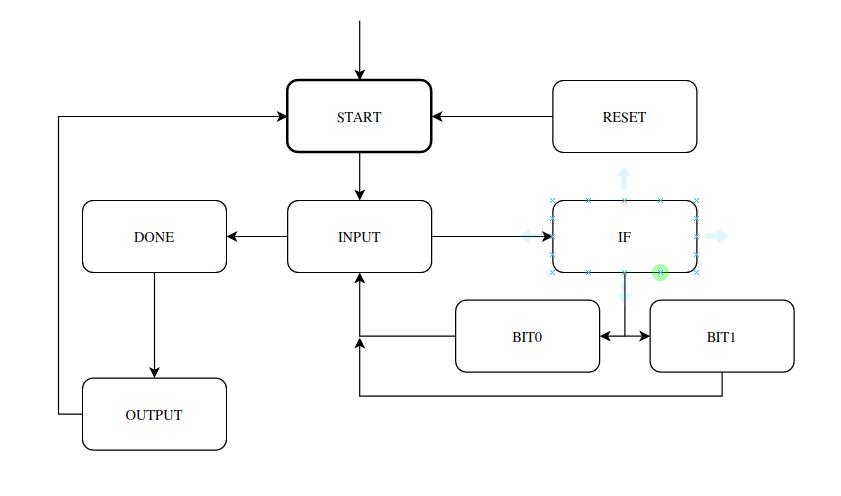
\includegraphics[height=11cm, width=15cm]{media/bmul_FSM}}
	 \caption{FSM for the binary multiplier module}
	\end{center}
\end{figure}
\clearpage
\begin{figure}[h!]
	\begin{center}
	 \fbox{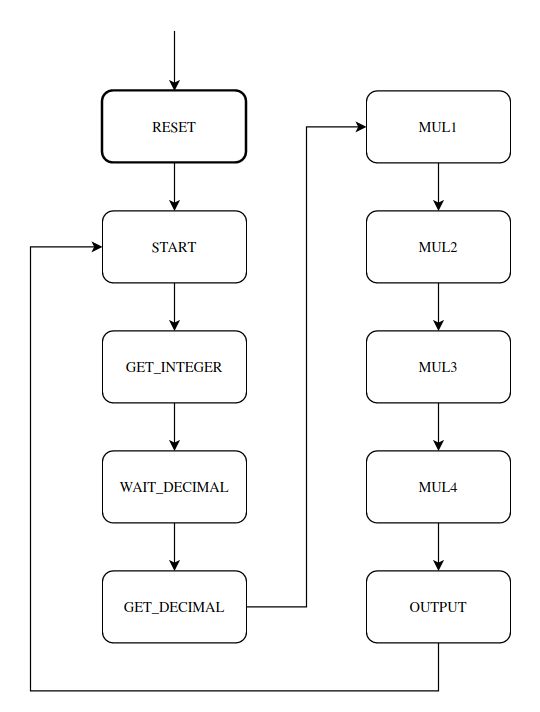
\includegraphics[height=17cm, width=13cm]{media/mmul_FSM}}
	 \caption{FSM for the matrix multiplier module}
	\end{center}
\end{figure}

Please refer to the code for both EFSM's, they were not included for size issues.

\section{FPGA Synthesis}
\begin{figure}[h!]
	\begin{center}
	 \fbox{\includegraphics[height=17cm, width=13cm]{media/synth_result}}
	 \caption{Result of the synthetization of the modules on the FPGA of reference ()}
	\end{center}
\end{figure}


\end{document}